\subsection{Nachbearbeitung der Vorhersagen}
\label{sec:Nachbearbeitung}
Mit dem trainierten Modell können nun Vorhersagen erzeugt werden.
In \autoref{lst:Prediction} ist dieser Prozess anhand eines zufälligen Beispiels aus den Validierungsdaten gezeigt.

\begin{code}
\begin{minted}[
    linenos,
    numbersep=10pt,
    gobble=0,
    frame=lines,
    framesep=2mm]{python}
def predict_random_example(model, val_dataset):
    example = val_dataset[np.random.choice(range(len(val_dataset)), size=1)[0]]
    x = np.expand_dims(example[0:-1, ...], axis=0)
    y_true = np.squeeze(example[-1, ...])
    y_pred = np.squeeze(model.predict(x))

    return y_true, y_pred
\end{minted}
\captionof{listing}{Erzeugung einer Vorhersage anhand der Validierungsdaten}
\label{lst:Prediction}
\end{code}

Dafür wird in Zeile 1 zunächst eine zufällige Sequenz von 17 Frames aus den Validierungsdaten ausgewählt.
In Zeile 2 und 3 wird die Sequenz in die Eingabe- und Zieldaten unterteilt, die dann jeweils in die richtige Form gebracht werden.
Die eigentliche Vorhersage findet dann in Zeile 5 statt, wo sie durch \emph{model.predict(x)} ausgeführt wird.
Die Arrays \emph{y\_true} und \emph{y\_pred} enthalten nun die Wahren und die vorhergesagten Ergebnisse und haben die Form $(50,~50)$.
In \autoref{fig:PredExProb} sind zwei Beispiele für Vorhersagen grafisch dargestellt.

\begin{figure}[h]
    \centering
    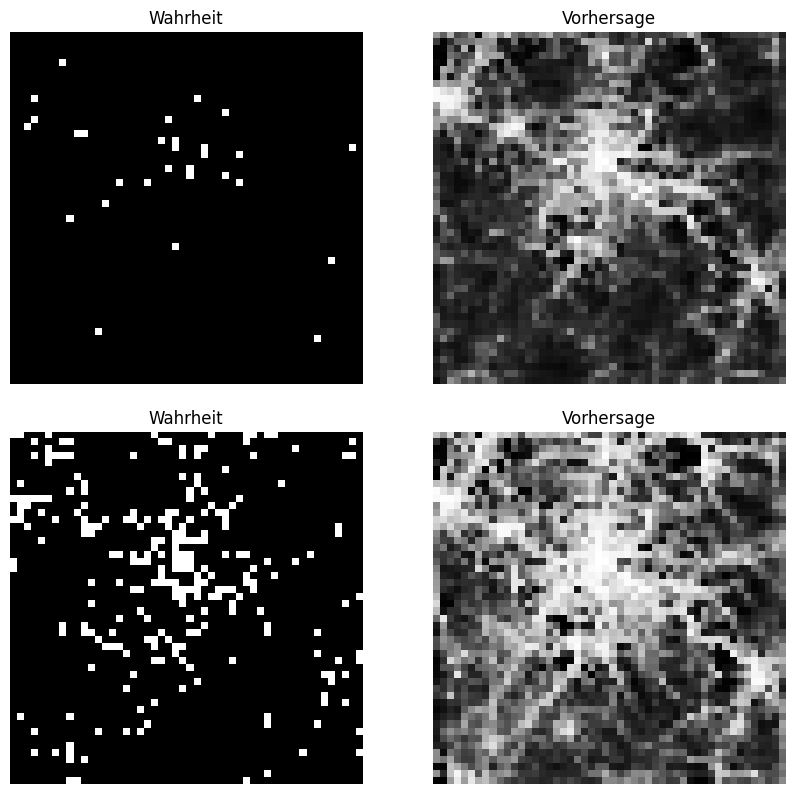
\includegraphics[width=1.0\textwidth,height=12cm,keepaspectratio=true]{content/images/PredExProb.png}
    \caption{Beispiele für Vorhersagen des trainierten Modells (rechts) im Vergleich zur Realität (links)}
    \label{fig:PredExProb}
\end{figure}

Links im Bild sieht man die realen Standorte der mobilen Radarkontrollen.
Rechts hingegen ist die Ausgabe des \acrshortpl{nn} dargestellt.
Je dunkler die Pixel, desto geringer ist der Zahlenwert und umgekehrt.
Zunächst kann man leicht erkennen, dass nicht alle Pixel schwarz sind, sondern dass ein weiter Bereich an Zahlenwerten abgedeckt wird.
Das spricht dafür, dass die gewichtete Verlustfunktion ihren Zweck erfüllt.
Als Nächstes ist erkennbar, dass das Modell scheinbar teilweise das Straßennetz erlernt hat.
In den Vorhersagen sind große Straßen als Linien und große Städte als Cluster deutlich erkennbar.
Dies ist durchaus nachvollziehbar, da die Radarkontrollendichte hier besonders hoch ist.
Dadurch stellt sich jedoch die Frage, ob die Vorhersage des Modells überhaupt maßgeblich von der Eingabe abhängig ist.
Dafür spricht jedenfalls der Unterschied zwischen dem oberen und unteren Beispiel.
Im oberen Beispiel sind in der Realität deutlich weniger Radarkontrollen vorhanden als im unteren Beispiel.
Das könnte beispielsweise dadurch zustande kommen, dass das obere Beispiel von einem Samstag oder Sonntag stammt.
In der bereits diskutierten \autoref{fig:AnzahlNachWochentag} ist schließlich deutlich zu erkennen, dass es am Wochenende deutlich weniger Radarkontrollen gibt als unter der Woche.
Auch die Vorhersage spiegelt diesen Sachverhalt wieder.
Während die Vorhersage im oberen Beispiel viele dunkle Pixel enthält, ist die Vorhersage im unteren Beispiel insgesamt deutlich heller, das Modell geht also insgesamt von einer höheren Wahrscheinlichkeit für mobile Radarkontrollen aus.
% TODO: Vergleich von gleichen Wochentagen? Auf später verweisen?

Zuletzt ist noch eine offensichtliche Tatsache anzumerken, die aber dennoch wichtig ist, und zwar die Beschaffenheit der Ausgabe des Modells.
Jedes Pixel wird als Zahlenwert zwischen 0 und 1 ausgegeben.
Das liegt an der Aktivierungsfunktion \emph{Sigmoid} des letzten Layers, die die Zahlengerade auf den Bereich zwischen 0 und 1 abbildet.
Der Bereich zwischen 0 und 1 legt nahe, dass die Ausgabe des Modells als Wahrscheinlichkeitskarte angesehen werden kann.
Nun stellt sich die Frage, ob die Ausgabe so belassen werden sollte oder ob sie noch nachverarbeitet werden sollte.
Hierzu gibt es zwei relevante Aspekte: die praktische Nutzbarkeit und die Performanceevaluierung.
Zur Performanceevaluierung muss beachtet werden, dass die Problemstellung bisher als Binärklassifizierung angesehen wird,
Daher muss die Ausgabe zur Evaluierung wie auch die Eingabe eine Binärklassifizierung sein.
Nur so kann bestimmt werden, wie viele Rasterzellen richtig Klassifiziert werden.
Im Bezug auch die praktische Nutzbarkeit ist es durchaus möglich, das Ergebnis als Wahrscheinlichkeit zu belassen.
Jedoch hat diese Vorgehensweise den Nachteil, dass eine Wahrscheinlichkeit unter Umständen schwer einzuschätzen sein kann, besonders in der Hektik des Straßenverkehrs.
Daher bietet es sich an, die ausgegebenen Wahrscheinlichkeiten in mehrere Gefahrenstufen zu unterteilen, die einfach verständlich sind.
Diese Gefahrenstufen könnten beispielsweise \emph{niedrig}, \emph{mittel}, \emph{hoch} und \emph{sehr hoch} heißen.

Unabhängig davon, ob die Wahrscheinlichkeiten als Binärklassifizierung in zwei Stufen aufgeteilt werden soll oder als Gefahrenangabe in mehrere, stellt sich die Frage, wo die Grenzen gesetzt werden sollten.
Eine gute und einfach zu interpretierende Möglichkeit ist die Entscheidung nach Perzentil.
In diesem Fall beziehen sich Perzentile auf die Verteilung der Rasterzellenwerte.
Die 90. Perzentilgrenze liegt beispielsweise so, dass 90\,\% aller Rasterzellen einen Wert unter dieser Grenze haben.
Bei der Wahl der Perzentilgrenze hat im Fall einer Binärklassifizierung eine große Auswirkung auf das Ergebnis.
Dies soll in \autoref{fig:PredExPercentile} verdeutlicht werden.

\begin{figure}[h]
    \centering
    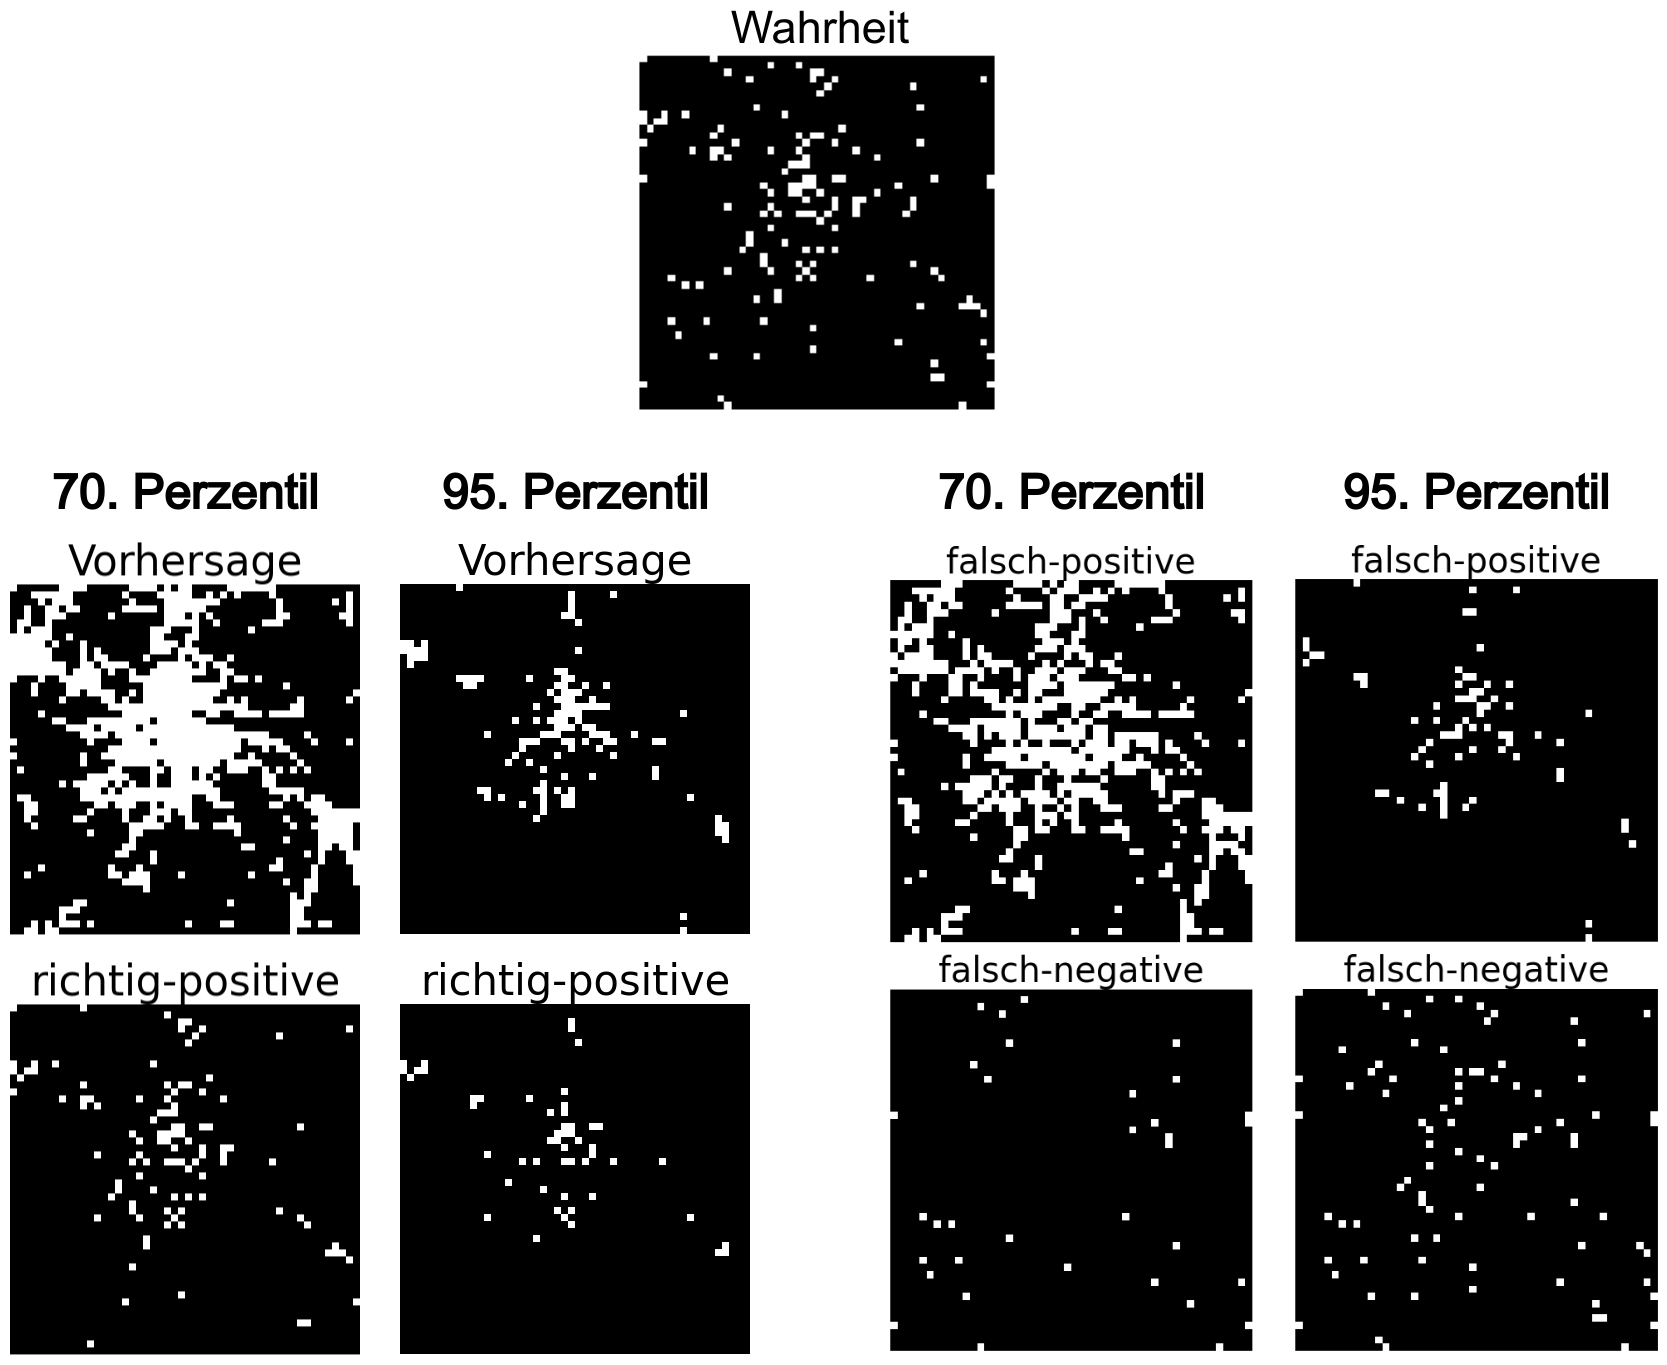
\includegraphics[width=1.0\textwidth,height=12cm,keepaspectratio=true]{content/images/PredExPercentile.png}
    \caption{Auswirkung der Perzentilgrenze auf die Vorhersage im Fall einer Binärklassifizierung}
    \label{fig:PredExPercentile}
\end{figure}

In der Abbildung ist als Beispiel eine Vorhersage bei zwei verschiedenen Perzentilgrenzen zu sehen.
Dabei zeigt das obere Bild die Grundwahrheit.
Unten ist die Vorhersage je für die 70. und 95. Perzentilgrenze dargestellt.
Außerdem ist die Vorhersage jeweils in die richtig-positiven, falsch-positiven und falsch-negativen aufgeschlüsselt.
Im Einklang mit der Definition der Perzentilgrenze ist beim Vergleich der Vorhersagen offensichtlich, dass mit der 70. Perzentilgrenze deutlich mehr Rasterzellen als "`positiv"' eingestuft werden als mit der 95. Perzentilgrenze.
Dies hat zur Folge, dass mit der 70. Perzentilgrenze mehr der tatsächlich positiven Rasterzellen korrekt vorhergesagt werden.
Jedoch resultieren daraus auch deutlich mehr falsch-positive.
Stellt man sich dieses Szenario in der Praxis vor, würden Benutzer relativ häufit gewarnt werden, obwohl keine akute Gefahr für Radarkontrollen besteht.
Es lässt sich jedoch argumentieren, dass es in der Praxis wichtiger ist, dass vor so vielen tatsächlich positiven Rasterzellen gewarnt werden sollte wie möglich, auch wenn dadurch Fehlwarnungen häufiger werden.
In \autoref{fig:PredExPercentile} sind bisher nur Beispiele für zwei konkrete Perzentilgrenzen dargestellt.
Für eine genauere Analyse sind jedoch Werte über alle Perzentilgrenzen interessant.
Diese sind als Graphen für dasselbe Beispiel in \autoref{fig:PredExGraphs} dargestellt.

\begin{figure}[h]
    \centering
    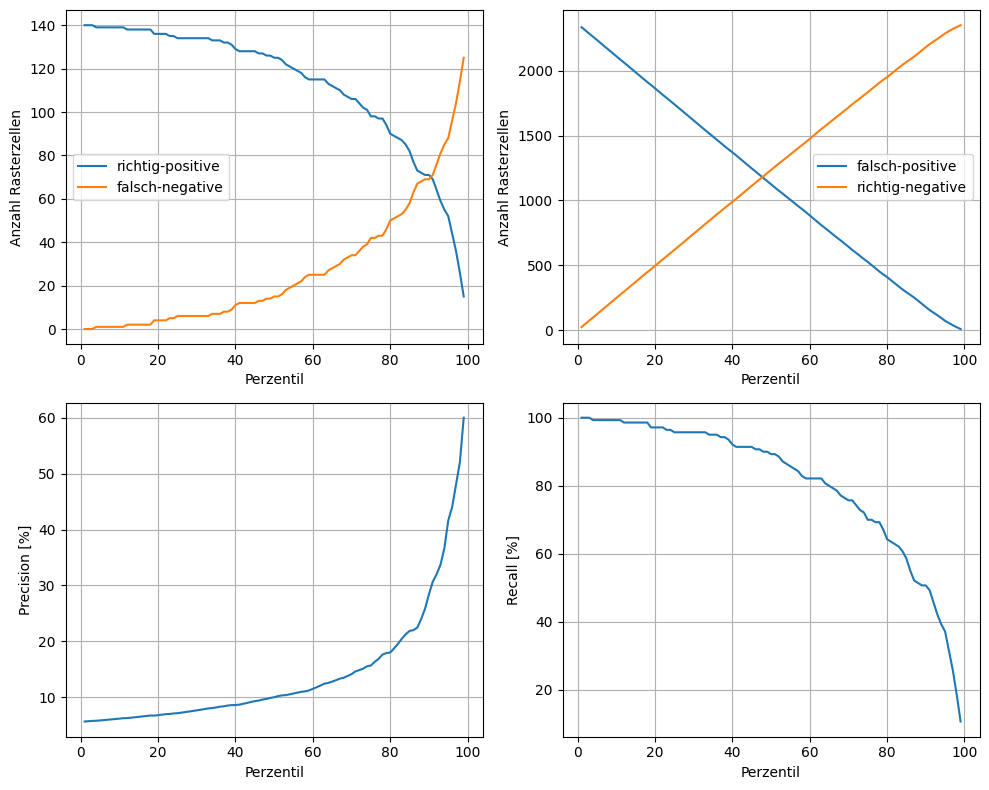
\includegraphics[width=1.0\textwidth,height=12cm,keepaspectratio=true]{content/images/PredExGraphs.png}
    \caption{Verschiedene Metriken einer Beispielvorhersage über Perzentilgrenzen von 1\,\% bis 99\,\%}
    \label{fig:PredExGraphs}
\end{figure}

In den oberen beiden Graphen sind die Kennzahlen, die oben schon für zwei Perzentilgrenzen analysiert wurden, über alle Perzentilgrenzen aufgetragen.
Für die Betrachtung ist wichtig zu wissen, dass es insgesamt 2500 Rasterzellen gibt, von denen in diesem Beispiel in der Realität 140 "`positiv"' sind.
Dies wird auch deutlich, wenn man die linken Enden der Graphen betrachtet.
Bei der nullten Perzentilgrenze werden per Definition alle Zellen als "`positiv"' markiert, weshalb dort auch die Anzahl der richtig-positiven maximal ist.
Jedoch ist dort auch die Anzahl der falsch-positiven maximal.
Aufgrund der unbalancierten Verteilung der positiven Rasterzellen verhält sich die richtig-positiven- und falsch-negativen-Rate über die Perzentligrenzen hinweg exponentiell, während sich die falsch-positiven- und richtig-negativen-Rate annähernd linear verhält.
Zur intuitiveren Bewertung der Perzentligrenzen sind die absoluten Zahlen wenig aussagekräftig, zumal sie sich bei verschiedenen Beispielen unterschiedlich verhält.
Daher gibt es verschiedene Metriken, die die absoluten Werte zueinander ins Verhältnis setzen.
Diese werden in \cite{ImbalancedData} beschrieben.
Die einfachste solche Metrik ist die Genauigkeit, die den Anteil der richtig klassifizierten Elemente darstellt, es gilt also
$$
\text{Genauigkeit} = \frac{\text{Korrekt klassifizierte Elemente}}{\text{Gesamtanzahl der Elemente}}.
$$
In \autoref{sec:ModellDefinition} wurde jedoch bereits erörtert, warum die Genauigkeit für unbalancierte Daten nicht aussagekräftig ist.
Deulich hilfreicher sind die Metriken \emph{Precision} und \emph{Recall}.
Precision ist nach \cite{ImbalancedData} der Anteil der positiv vorhergesagten Elemente, die auch in der Realität "`positiv"' sind, es gilt also
$$
\text{Precision} = \frac{\text{richtig-positive}}{\text{richtig-positive + falsch-positive}}.
$$
Recall gibt hingegen an, welcher Anteil der tatsächlich positiven Elemente auch als "`positiv"' erkannt werden.
Hier gilt somit
$$
\text{Recall} = \frac{\text{richtig-positive}}{\text{richtig-positive + falsch-negative}}.
$$
Um diese Metriken genauer zu verstehen ist es hilfreich zu betrachten, wann sie 100\,\% betragen.
Damit die Precision 100\,\% beträgt, darf es keine falsch-positiven geben.
Somit ist die Precision ein Maß dafür, wie präzise \emph{nur} die tatsächlich Positiven erkannt werden.
Wichtig ist hierbei anzumerken, dass die Precision nichts darüber aussagt, wie viele der tatsächlich Positiven erkannt werden.
Die Precision könnte also 100\,\% betragen, obwohl nur wenige Prozent der tatsächlich Positiven erkannt werden.
Wichtig ist nur, dass es keine falsch-positiven gibt.
Genau andersherum ist es nun beim Recall.
Der Recall beträgt genau dann 100\,\%, wenn es keine falsch-negativen gibt.
Es müssen also alle tatsächlich positiven Elemente erkannt werden.
Dabei ist es jedoch unerheblich, wie viele in der Realität negativen Elemente zusätzlich noch als "`positiv"' erkannt werden.

Insgesamt ist also klar, dass bei der Wahl der Perzentilgrenze zwischen Precision und Recall abgewogen werden muss.
In \autoref{fig:PredExGraphs} sind Precision und Recall in den unteren beiden Graphen für das konkrete Beispiel dargestellt.
Anhand des Precision-Graphs ist zu erkennen, dass selbst mit einer Perzentilgrenze von 99\,\% keine Precision über 60\,\% möglich ist.
Es gibt also immer eine gewisse, nicht zu vernachlässigende Anzahl an falsch-positiven.
Außerdem ist erkennbar, dass die Precision-Kurve bei Perzentilgrenzen gegen 99\,\% sehr stark ansteigt.
Die Rasterzellen, die einen Wert in diesem Bereich haben, sind also mit großer Wahrscheinlichkeit tatsächlich "`positiv"'.
Im Bezug auf den Anwendungsfall der Vorhersage von mobilen Radarkontrollen hat die Recall-Kurve eine nochh größere Bedeutung, da möglichst viele tatsächlich vorhandenen Radarkontrollen in der Vorhersage vorhanden sein sollten.
Jedoch bleibt es eine Abwägung zwischen Precision und Recall.
Daher bietet es sich an, beide Metriken in einem Graph in Relation zueinander zu setzen.
Diesen Graph nennt man \acrfull{prc}.
Die \acrshort{prc} der bisher verwendeten Beispielvorhersage ist in \autoref{fig:PredExGraphsPRC} links dargestellt.

\begin{figure}[h]
    \centering
    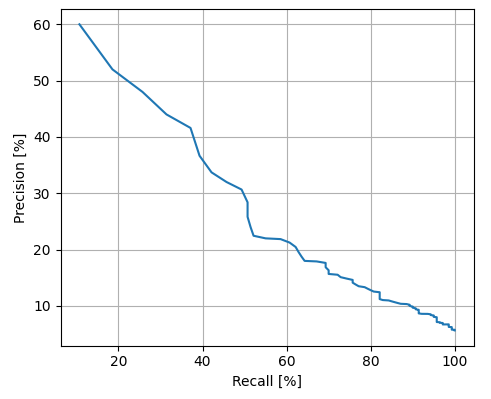
\includegraphics[width=0.7\textwidth,height=8cm,keepaspectratio=true]{content/images/PredExGraphsPRC.png}
    \caption{\acrfull{prc} einer Beispielvorhersage}
    \label{fig:PredExGraphsPRC}
\end{figure}

An diesem Graphen kann abgelesen werden, welche Precision bei welchem Recall erreichbar ist und umgekehrt.
Soll beispielsweise ein Recall von 70\,\% erreicht werden, entspricht dies einer Precision von ca. 15\,\%.
In Worten werden also 70\,\% aller Rasterzellen korrekt vorhergesagt, die tatsächlich eine Radarkontrolle beinhalten, jedoch enthalten nur 15\,\% aller als "`positiv"' vorhergesagten Rasterzellen tatsächlich eine Radarkontrolle.
Wenn die \acrshort{prc} für den gesamten Validierungsdatensatz erstellt wird, eignet sie sich auch dazu, die Performance verschiedener Modelle zu vergleichen.
Falls ein Modell besser performt als ein anderes, liegt die \acrshort{prc} dieses Modells eher weiter oben rechts.
Es ergeben sich also insgesamt größere Precision-Recall-Paare.

Die \acrshort{prc} kann nun gemeinsam mit den einzelnen Graphen von Precision und Recall verwendet werden, um geeignete Perzentilgrenzen für eine Gefahreneinstufung auszuwählen.
Für die Einteilung in die vier Gefahrenstufen \emph{niedrig}, \emph{mittel}, \emph{hoch} und \emph{sehr hoch} müssen drei Perzentilgrenzen ausgewählt werden.
Für die Grenze, ab der die Gefahrenstufe \emph{mittel} gelten soll, scheint das 60. Perzentil ein guter Wert zu sein.
Dies entspricht einem Recall von ca. 82\,\% und einer Precision von ca. 12\,\%.
Der Recall-Wert bedeutet, dass nur 18\,\% der tatsächlichen Radarkontrollen (fälschlicherweise) auf die Gefahrenstufe \emph{niedrig} fallen.
Die Precision ist jedoch nicht sonderlich hoch.
Es befinden sich folglich sehr viele falsch-positive in der Gefahrenstufe \emph{mittel}.
Die nächste Gefahrenstufe (für die Gefahrenstufe \emph{hoch}) kann beim 85. Perzentil angelegt werden.
Hier beträgt der Recall ca. 60\,\% und die Precision ca. 23\,\%.
Die Precision hat sich demnach im Vergleich zur Gefahrenstufe \emph{mittel} fast verdoppelt, während der Recall nur um ein Viertel geringer geworden ist.
Bei der Gefahrenstufe \emph{sehr hoch} sollte sich das Modell sehr sicher sein, dass sich in einer solchen Rasterzelle eine Radarkontrolle befindet.
Daher sollte eine Perzentilgrenze nahe 100\,\% gewählt werden, wie beispielsweise die 98. Perzentilgrenze.
Hier beträgt der Recall zwar nur noch ca. 10\,\%, die Precision jedoch ca. 55\,\%.
Statistisch befinden sich demnach in ca. der hälfte aller Rasterzellen der Gefahrenstufe \emph{sehr hoch} tatsächlich eine Radarkontrolle.

Werden die Gefahrenstufen mit unterschiedlichen Farben markiert, ergibt sich für das bisher verwendete Beispiel die in \autoref{fig:Gefahrenstufen} dargestellte Gefahrenkarte.

\begin{figure}[h]
    \centering
    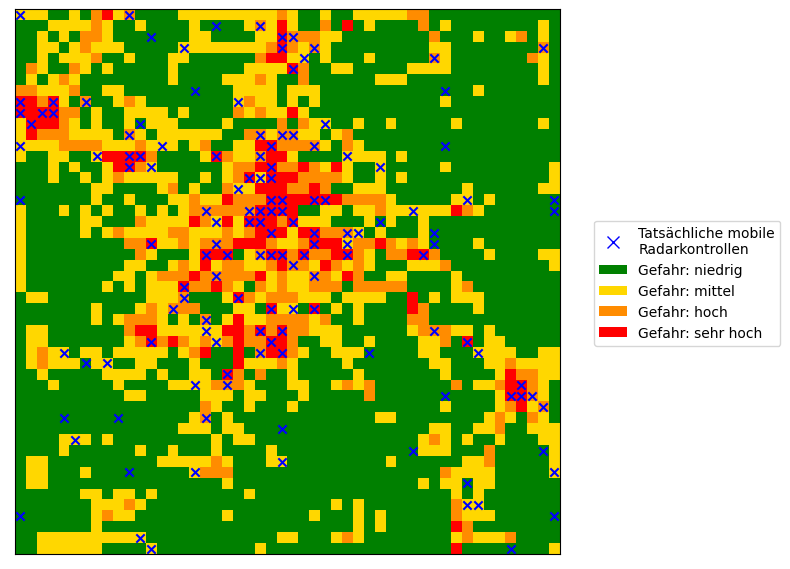
\includegraphics[width=0.7\textwidth,height=8cm,keepaspectratio=true]{content/images/Gefahrenstufen.png}
    \caption{Resultierende nachbearbeitete Vorhersage mit vier Gefahrenstufen im Vergleich zur Grundwahrheit}
    \label{fig:Gefahrenstufen}
\end{figure}

Außerdem sind in der Abbildung die tatsächlichen Radarkontrollen mit einem Kreuz markiert.
Wird einem Autofahrer bei jedem Rasterzellenwechsel die neue Gefahrenstufe mitgeteilt, kann dieser sie leicht einschätzen und sich entsprechend verhalten.
